\documentclass[a4paper,12pt]{article}
\usepackage[a4paper,top=3cm,bottom=2cm,left=3cm,right=3cm,marginparwidth=1.75cm]{geometry}
\usepackage[brazil]{babel}
\usepackage[T1]{fontenc}
\usepackage[utf8]{inputenc}
\usepackage{amsmath}
\usepackage{MnSymbol}
\usepackage{wasysym}
\usepackage{hyperref}
\usepackage{color}
\definecolor{Blue}{rgb}{0,0,0.9}
\definecolor{Red}{rgb}{0.9,0,0}
\usepackage{esvect}
\usepackage{graphicx}
\usepackage{float}
\usepackage{indentfirst}
\usepackage{caption}
\usepackage{blkarray}
\newcommand\Mark[1]{\textsuperscript#1}
\usepackage{pgfplots}
\usepackage{amsfonts}
\title{Relatório de Laboratório 2}
\author{Guilherme Philippi, Carlos Eduardo dos Santos Junior}
\begin{document}
\maketitle
\tableofcontents

\section{Introdução}

Este relatório tem como objetivo apresentar soluções de exercícios envolvendo grafos.

Utilizou-se o software PIPE (Platform Independent Petri net Editor) \cite{dias2007ferramentas} para modelar e simular as soluções propostas, assim como segue na próxima seção.

\section{Desenvolvimento}
Descrever de forma mais detalhada o problema.
Apresentar a solução proposta pela equipe.
Discorrer sobre a solução (por exemplo, explicar com detalhes os pontos mais
importantes).

\begin{figure}[H]
	\begin{center}
		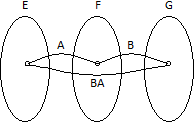
\includegraphics[width=0.4\linewidth]{compfunc.png}
	\end{center}
	\caption{Transformação linear composta BA}
	\label{fig:compfunc}
\end{figure}

Atenção: Se mais de uma ou atividade foi realizada no laboratório repetir a sequência
anterior (da Seção 3) para cada atividade.

\section{Considerações Finais}
Apresentar as considerações finais sobre o trabalho. Se o objetivo foi alcançado ou não,
o que foi aprendido, dificuldades encontradas, etc.

\newpage
\phantomsection
\addcontentsline{toc}{section}{Referências}

\bibliographystyle{unsrt}
\bibliography{references}

\end{document}
